\documentclass[border=10pt]{standalone}
\usepackage[svgnames]{xcolor}
\usepackage{amsmath}
\usepackage{pgfplots}
\pgfplotsset{compat=newest}
\usepackage[sfdefault]{FiraSans}
\usepackage{FiraMono}
\renewcommand*\familydefault{\sfdefault}
\begin{document}
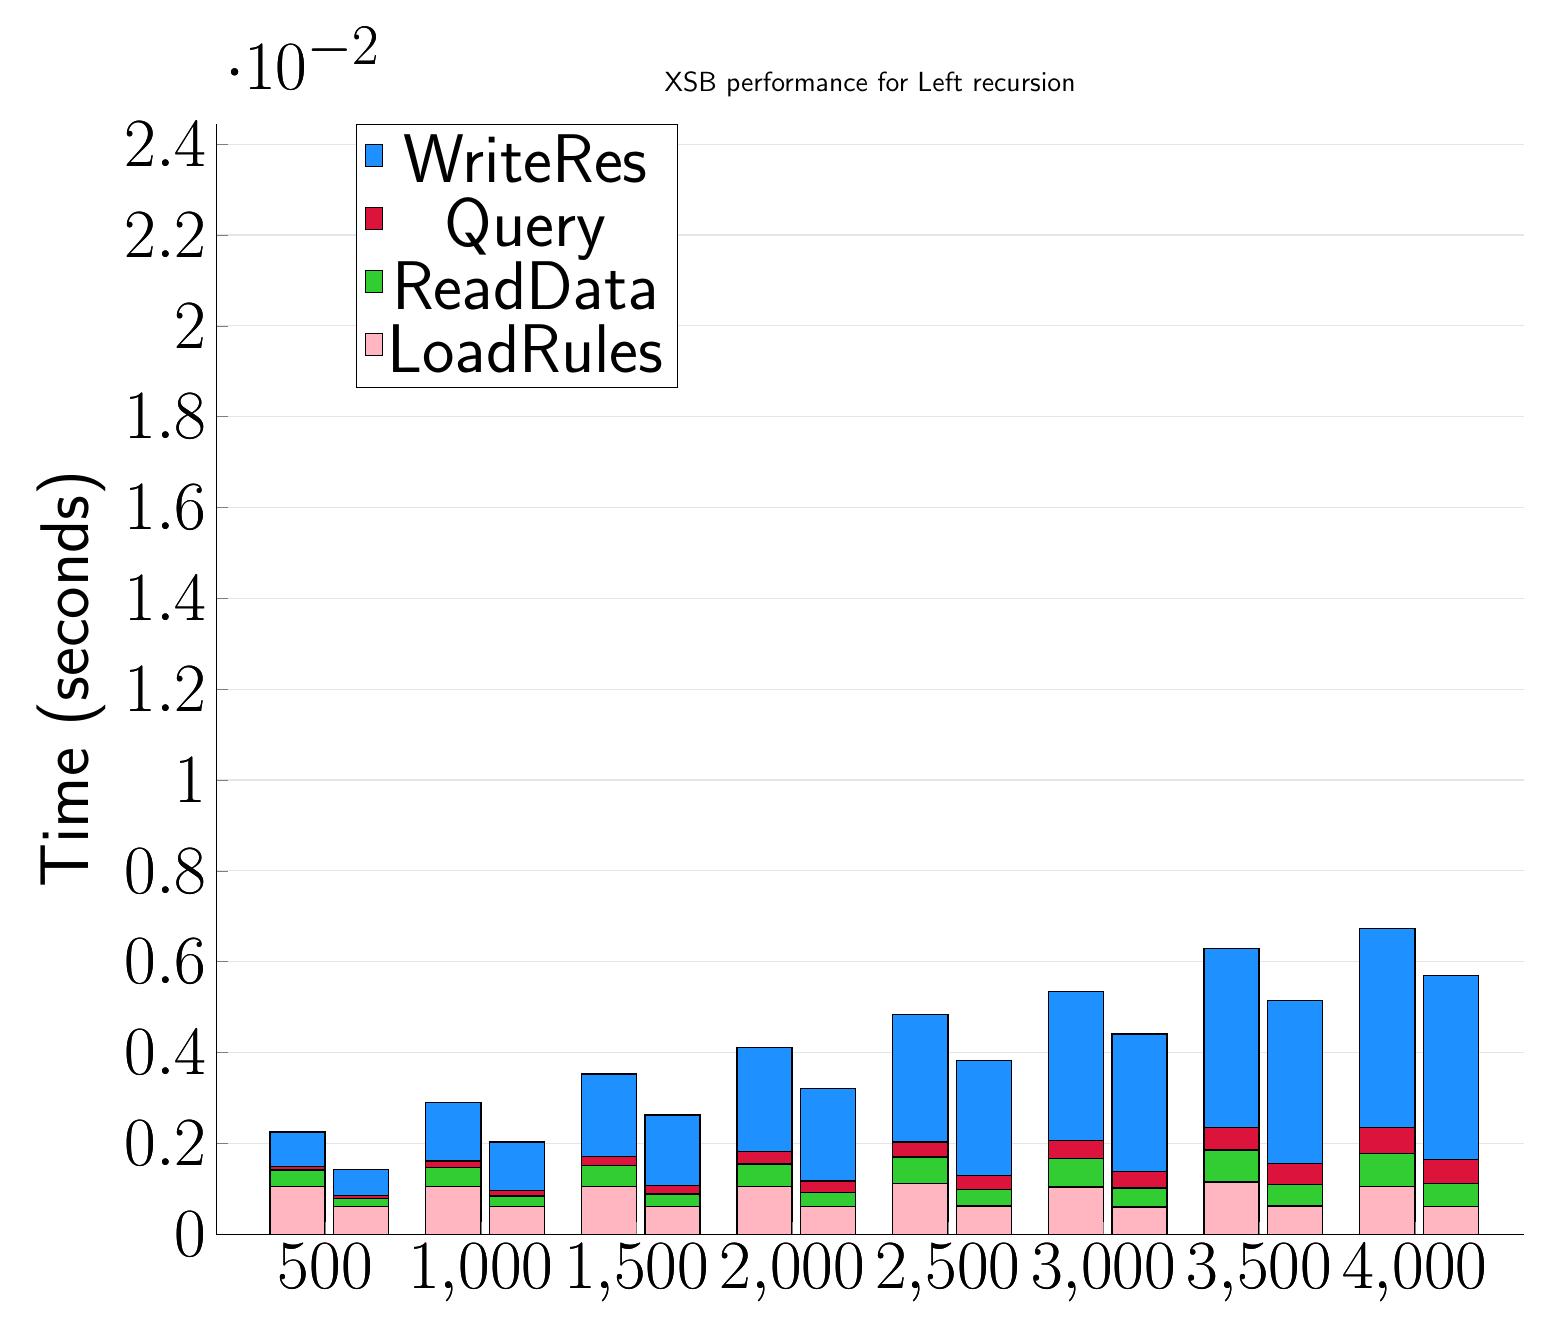
\begin{tikzpicture}
\begin{axis}[
   ybar stacked,
   title={XSB performance for Left recursion},
   bar shift=-10pt,
   width=1.5\textwidth,
   bar width=0.7cm,
   ymajorgrids, tick align=inside,
   major grid style={draw=gray!20},
   xtick=data,
   ymin=0, ymax=0.02445413589477539,
   axis x line*=bottom,
   axis y line*=left,
   enlarge x limits=0.1,
   legend style={
       at={(0.23, 1)},
       anchor=north,
       legend columns=1,
       font=\Huge,
   },
   ylabel={Time (seconds)},
   label style={font=\Huge},
   tick label style={font=\Huge},
]
\addlegendimage{fill=DodgerBlue, draw=black, line width=0.2pt}
\addlegendentry{WriteRes}
\addlegendimage{fill=Crimson, draw=black, line width=0.2pt}
\addlegendentry{Query}
\addlegendimage{fill=LimeGreen, draw=black, line width=0.2pt}
\addlegendentry{ReadData}
\addlegendimage{fill=LightPink, draw=black, line width=0.2pt}
\addlegendentry{LoadRules}
\addplot +[fill=LightPink, draw=black, line width=0.5pt] coordinates {
    (500, 0.001044964790344238)
    (1000, 0.001052927970886229)
    (1500, 0.001054835319519044)
    (2000, 0.001046657562255859)
    (2500, 0.0011100530624389648)
    (3000, 0.001041793823242186)
    (3500, 0.00115220546722412)
    (4000, 0.001050567626953125)
};
\addplot +[fill=LimeGreen, draw=black, line width=0.5pt] coordinates {
    (500, 0.0003692388534545899)
    (1000, 0.00041961669921875016)
    (1500, 0.0004636526107788086)
    (2000, 0.0004991054534912109)
    (2500, 0.0005873441696166991)
    (3000, 0.0006246566772460938)
    (3500, 0.0007035732269287108)
    (4000, 0.0007249116897583008)
};
\addplot +[fill=Crimson, draw=black, line width=0.5pt] coordinates {
    (500, 7.410049438476564e-05)
    (1000, 0.0001354217529296875)
    (1500, 0.00019721984863281262)
    (2000, 0.00027143955230712885)
    (2500, 0.0003317832946777344)
    (3000, 0.00039854049682617185)
    (3500, 0.0005000114440917968)
    (4000, 0.0005729436874389648)
};
\addplot +[fill=DodgerBlue, draw=black, line width=0.5pt] coordinates {
    (500, 0.0007595062255859374)
    (1000, 0.0012954711914062494)
    (1500, 0.0018132925033569332)
    (2000, 0.0022909402847290034)
    (2500, 0.0028038501739501955)
    (3000, 0.003282976150512696)
    (3500, 0.003929591178894043)
    (4000, 0.004381322860717773)
};
\end{axis}
\begin{axis}[
   ybar stacked,
   bar shift=13pt,
   width=1.5\textwidth,
   bar width=0.7cm,
   ymajorgrids, tick align=inside,
   major grid style={draw=none},
   xtick=data,
   ymin=0, ymax=0.02445413589477539,
   axis x line*=none,
   axis y line*=none,
   enlarge x limits=0.1,
   label style={font=\Huge},
   tick label style={font=\Huge},
]
\addplot +[fill=LightPink, draw=black, line width=0.5pt] coordinates {
    (500, 0.0006053000000000001)
    (1000, 0.0006111999999999997)
    (1500, 0.0006153)
    (2000, 0.0006115999999999997)
    (2500, 0.0006187999999999999)
    (3000, 0.0006029999999999999)
    (3500, 0.0006214)
    (4000, 0.0006072000000000004)
};
\addplot +[fill=LimeGreen, draw=black, line width=0.5pt] coordinates {
    (500, 0.0001807999999999999)
    (1000, 0.00022850000000000049)
    (1500, 0.0002712999999999999)
    (2000, 0.00031089999999999997)
    (2500, 0.00036459999999999997)
    (3000, 0.0004112000000000003)
    (3500, 0.0004664999999999996)
    (4000, 0.0005027999999999996)
};
\addplot +[fill=Crimson, draw=black, line width=0.5pt] coordinates {
    (500, 6.699999999999985e-05)
    (1000, 0.0001253999999999999)
    (1500, 0.0001862999999999995)
    (2000, 0.00025079999999999997)
    (2500, 0.0003081000000000002)
    (3000, 0.00037329999999999953)
    (3500, 0.0004655999999999996)
    (4000, 0.0005394999999999999)
};
\addplot +[fill=DodgerBlue, draw=black, line width=0.5pt] coordinates {
    (500, 0.0005673000000000003)
    (1000, 0.0010644)
    (1500, 0.0015532000000000007)
    (2000, 0.0020402000000000003)
    (2500, 0.0025369000000000004)
    (3000, 0.0030177000000000003)
    (3500, 0.0035862999999999997)
    (4000, 0.0040451)
};
\end{axis}
\end{tikzpicture}

\end{document}
